\section{Software Agents}
\label{sec:agents}

\begin{figure}
    \centering
    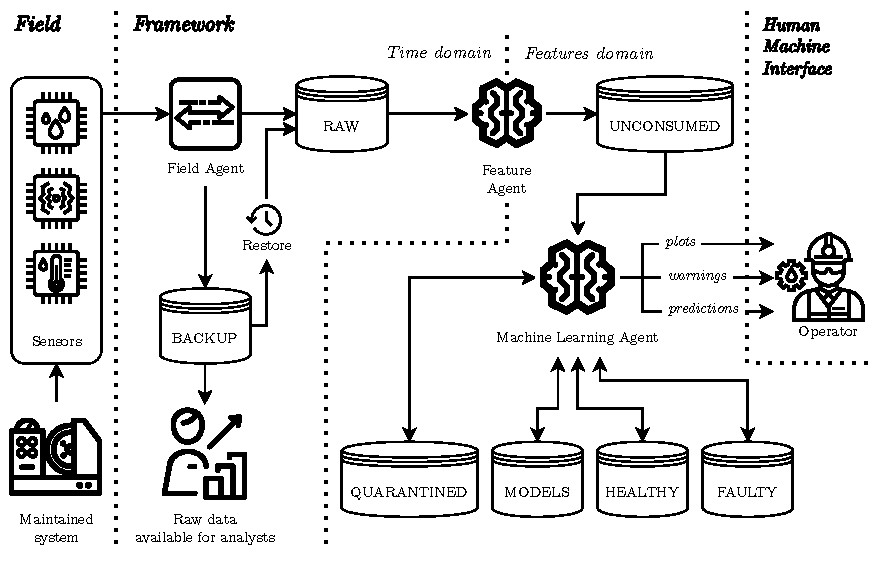
\includegraphics[width=\textwidth]{images/Framework/Framework_structure.pdf}
    \caption{Framework logical structure}
    \label{fig:Framework_structure}
\end{figure}

In the previous sections, the software agents were mentioned as the main actors in the framework. This section will provide a more detailed description of the software agents, their role and their interaction with the environment and the data, following the flow from the hardware through the time-series, the feature domain to the \gls{ml} algorithms. The reference layout is the one in \autoref{fig:Framework_structure}. 

Software \gls{glo:agent}s are autonomous programs that perform a specific task in a cycle. In the proposed \texttt{python} implementation, the agents are classes that are instanced and run in a loop.

\subsection{Field Agent}
\label{subsec:FieldAgent}
\begin{figure}
    \centering
    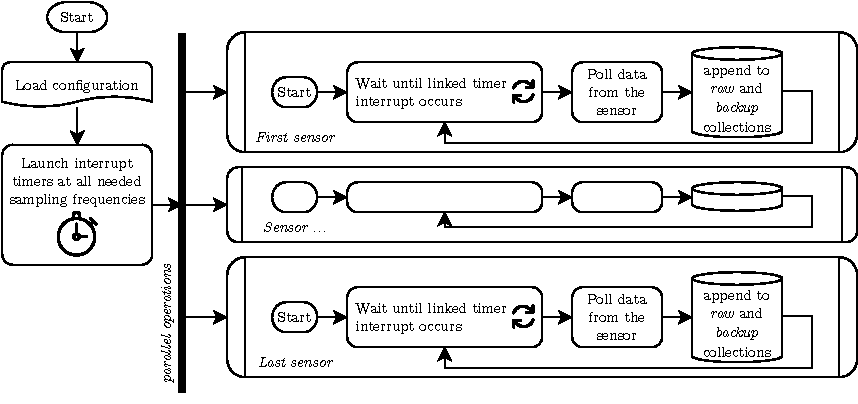
\includegraphics[scale=1]{images/Framework/Field_Agent_flowchart.pdf}
    \caption{Field Agent flowchart}
    \label{fig:Field_Agent_flowchart}
\end{figure}

The \gls{glo:fieldagent} is the interface between the hardware and the software. It is responsible for the acquisition of the data from the sensors and the communication with the database. Since some features are related to the spectrum of the data, a precise and fixed sampling frequency is needed. Hence, the \gls{fieldAg} must incorporate a synchronization with the \gls{adc}. It stores data in the \emph{raw} collection and the \emph{backup} collection. In \autoref{fig:Field_Agent_flowchart}, the flow of operations are shown as a flowchart, emphasizing the importance of the synchronization with the \gls{adc}. This software agent has not been implemented in \texttt{python}, because the experimental validation of this work, as it will be described in \autoref{sec:Validation}, has been performed directly on the \gls{glo:edge} platform. During the tests on the publicly available datasets, an abstract version of the \gls{fieldAg} has been used, that reads the data from the \gls{csv} files.


\subsection{Feature Agent (FA)}
\label{subsec:FeatureAgent}
\begin{figure}
    \centering
    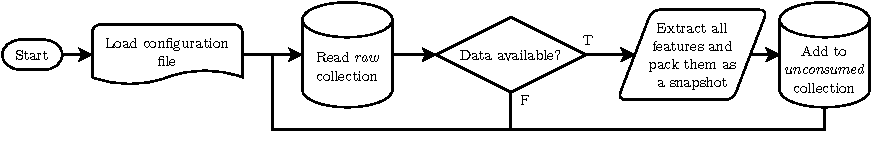
\includegraphics[width=\textwidth]{images/Framework/FA_flowchart.pdf}
    \caption{Feature Agent flowchart}
    \label{fig:FA_flowchart}
\end{figure}

The \gls{fa} is responsible for the feature extraction from the raw data. It reads the data from the \emph{raw} collection, extracts the features and stores them in the \emph{unconsumed} collection. The flow of operation is shown in \autoref{fig:FA_flowchart}. The \gls{fa} is implemented in \texttt{python} and it is a class that has been designed to be easily expandable and configurable. The methods implemented in the \gls{fa} class are shown in \autoref{tab:FA_methods}.


\begin{longtable}{p{0.4\textwidth}p{0.5\textwidth}}
    \caption{\gls{fa} class implemented methods\label{tab:FA_methods}}\\ 
    \toprule
    \textbf{Method} & \textbf{Description} \endfirsthead
    \hline
    readFromRaw & reads a snapshot from the raw collection and stores it in the instance self \\
    extractFeatures & extract all the features from the current snapshots, for all the sensors \\
    extractTimeFeautures & extract~mean,~rms, P2P, std, skewness and kurtosis, based on the config file for the specified sensor \\
    extractFreqFeautures & extract the wavelet coefficients for the specified sensor, up to the configured depth \\
    deleteFromraw & delete current snap record from the \emph{raw} collection \\
    writeToUnconsumed & write the extracted features to the \emph{unconsumed} collection \\
    initialize\_barPlotFeatures & initializes the bar plot of the features that is shown to the user \\
    barPlotFeatures & updates the bar plot with new features \\
    run & perform the agent operations in loop. idle until new data are available in \emph{raw} collection \\
    \bottomrule
\end{longtable}
    

\subsection{Machine Learning Agent (MLA)}
\label{subsec:MLA}
The \gls{mla} is responsible for the training and the evaluation of the \gls{ml} models. It reads the data from the \emph{unconsumed} collection, evaluates the snapshot and stores the result in the \emph{models} collection, it also constantly updates the information about the novelty or fault metric to the user. The flow of operation is shown in \autoref{fig:MLA_structure}. The methods implemented in the \gls{mla} class are shown in \autoref{tab:MLA_methods}.

This agent is designed to be configured as a \gls{nd} or \gls{fd} agent with just one hyperparameter. If it is instanced for \gls{nd}, it uses the healthy collection as a training dataset, if it is instanced for \gls{fd} it uses the faulty collection. The metric used to evaluate the snapshots is the novelty metric for \gls{nd} and the fault metric for \gls{fd}. According to the procedure defined in \autoref{alg:eval_new_snapshot}.

\begin{figure}[htbp]
    \centering
    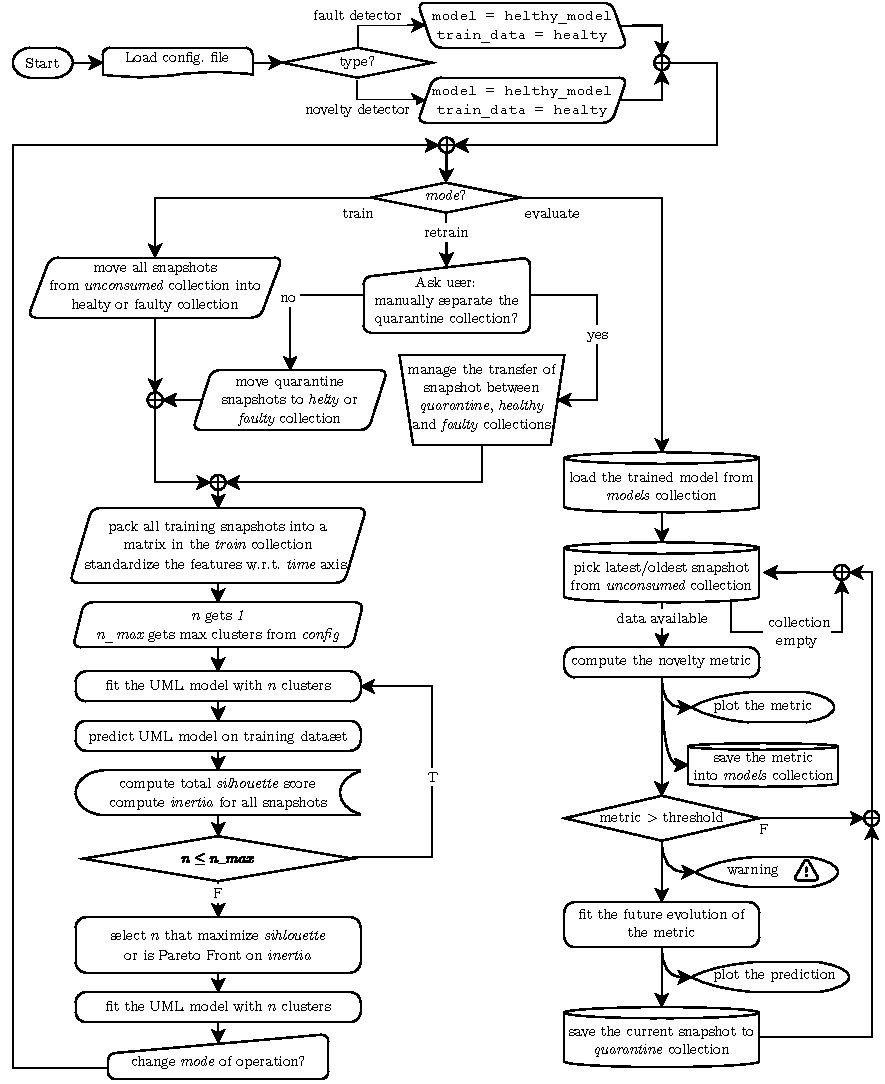
\includegraphics[width=\textwidth]{images/Framework/MLA.pdf}
    \caption{Machine Learning Agent flowchart. When it is instanced for \gls{nd}, the \gls{mla} uses the healthy collection as a training dataset, when it is instanced for \gls{fd} it uses the faulty collection.}
    \label{fig:MLA_structure}
\end{figure}


\begin{longtable}{p{0.4\textwidth}p{0.5\textwidth}}
    \caption{\gls{mla} class implemented methods\label{tab:MLA_methods}}\\ 
    \toprule
    \textbf{Method} & \textbf{Description} \endfirsthead 
    \hline
    run & run the \gls{mla} according to its current state \\
    evaluate & evaluate the current snapshot based on the novelty or the fault metric, according to the type of instance \\
    predict & fit the novelty metric with a degradation curve to predict the future evolution~ \\
    mark\_snap\_evaluated & set the evaluated flag to true for the current snapshot \\
    delete\_evaluated\_snap & remove the evaluated snapshots from the \emph{unconsumed} collection \\
    scale\_features & scales the features of the current snapshot according to the standard scaler used during the training procedure \\
    evaluate\_error & compute the novelty or fault metric for the current snapshot, according to the type of instance \\
    calculate\_train\_cluster\_dist & compute the radiuses of the clusters during the training procedure \\
    prepare\_train\_data & performs the preprocessing of the data before training the model \\
    pack\_train\_data & pack the training snapshot in a matrix \\
    \_\_move\_to\_train & move an entire collection of snapshots to the training collection \\
    standardize\_features & make all the features in the training matrix have zero mean and unitary variance \\
    save\_features\_limits & save the unscaled bounds of the training features \\
    save\_StdScaler & store the standard scaler instance in \gls{glo:pickle} into the database \\
    retrieve\_StdScaler & restore the standard scaler instance in \gls{glo:pickle} from the database \\
    save\_KMeans & store the model instance in \gls{glo:pickle}  \\
    retrieve\_KMeans & restore the model instance in \gls{glo:pickle}  \\
    \_append\_features & append the current features in a document \\
    train & performs the training of the clustering models \\
    evaluate\_silhouette & compute the silhouette score of the training set snapshots \\
    \_\_plot\_silhouette & plots the silhouette score against the number of clusters \\
    evaluate\_inertia & compute the inertia score of the training set snapshots \\
    \_\_plot\_inertia & plots the inertia score against the number of clusters \\
    packFeaturesMatrix & format all the training features as a matrix \\
    retrain & perform a new training of the models \\
    \bottomrule
    \end{longtable}
    
\newpage
\subsection{Configuration of the framework}
All the configurations described in this chapter are stored in the \texttt{config.yaml} file. This file is read by the agents at the beginning of their execution. The configuration file is divided into sections by topic: database, models etc. An example of a valid configuration file for the \gls{ims} dataset is shown in below.
\begin{minted}[
    gobble=4,
    frame=single,
    linenos,
    breaklines
  ]{yaml}
    Database:           # Database configuration
    URI:                mongodb://localhost:27017   # MongoDB URI
    db:                 Shaft                       # Database name
    collection:       # Collection configuration
      back:             BACKUP        # Backup collection name
      raw:              RAW           # Raw data collection name
      unconsumed:       UNCONSUMED    # Unconsumed data collection name
      healthy:          HEALTHY       # Healthy data collection name
      healthy_train:    HEALTHY_TRAIN # Healthy data collection name for training (some healthy data are not used if not novelty)
      quarantined:      QUARANTINED   # Quarantined data collection name
      faulty:           FAULTY        # Faulty data collection name
      faulty_train:     FAULTY_TRAIN  # Faulty data collection name for training (some faulty data are not used if not fault novelty)
      models:           MODELS        # Models collection name
    sensors:          # Expected sensors in the database
      Bearing 1 x:    # Sensor 1 name
        features:     # Features configuration
          wavPowers:    on            # Wavelet powers
          mean:         on            # Mean value
          rms:          on            # Root mean square
          peak:         on            # Peak to peak value
          std:          on            # Standard deviation
          skew:         on            # Skewness
          kurt:         on            # Kurtosis
      Bearing 1 y:    # Sensor 2 name
        features:     # Features configuration
          wavPowers:    on            # Wavelet powers
          mean:         on            # Mean value
          rms:          on            # Root mean square
          peak:         on            # Peak to peak value
          std:          on            # Standard deviation
          skew:         on            # Skewness
          kurt:         on            # Kurtosis
      ...:
      Bearing 4 y:    # Sensor n name
        features:     # Features configuration
          wavPowers:    on            # Wavelet powers
          mean:         on            # Mean value
          rms:          on            # Root mean square
          peak:         on            # Peak to peak value
          std:          on            # Standard deviation
          skew:         on            # Skewness
          kurt:         on            # Kurtosis
    wavelet:           # Wavelet packet transform configuration
      type:               db10          # Type of wavelet to use
      mode:               symmetric     # Mode of the packet transform
      maxlevel:           6             # Max level -> num of features = 2^level
    model:             # machine learning model configuration
      max_clusters:       100           # Max number of clusters
      max_iterations:     1000          # Max number of iterations
      error_queue_size:   1             # number of predictions parameters to keep in queue for plotting/predicting
      error_plot_size:    2000          # Size of the plotting queue
    novelty:           # Novelty/fault configuration
      threshold:          0.10          # Threshold for novelty / fault detection: relative percentage of the distance to the cluster w.r.t the max distance to the assigned cluster in the training set
      forecast_threshold: 0.8           # Threshold for novelty / fault prediction
      n_fit:              250           # Number of samples used to fit the prediction curve
      outlier_filter:     1             # Number of consecutive outliers to filter (1 means two outliers will be considered as novelty/fault)
      regressor:          exp           # Regressor to use for prediction: exp, scipy, poly. if exp uses a custom function, if scipy uses scipy.optimize.curve_fit, if poly fit polynomial of degree
    miscellanea:
      logpath:            C:\Users\JohnSmith\Documents\framework  # Path to the logs
\end{minted}

\subsection{Command Line Interface (CLI)}
\label{subsec:CLI}

To ease the interaction with the user, a \gls{cli} has been implemented. It relies on the \texttt{click} and \texttt{typer} libraries for \texttt{python}. The \gls{cli} allows the user to instance the agents, to configure the framework, to monitor the agents and to interact with the database. All the commands are provided with a help message that can be accessed by typing \texttt{--help} after the command, as shown in \autoref{fig:cli} for the command \texttt{run-machine-learning-agent}.
The commands implemented in the \gls{cli} are shown in \autoref{tab:CLI_commands}.

\begin{figure}[h!]
  \centering
  \includegraphics[width=\textwidth]{images/Framework/cli.png}
  \caption{Command Line Interface help message}
  \label{fig:cli}
\end{figure}

\begin{longtable}{p{0.4\textwidth}p{0.5\textwidth}}
    \caption{\gls{cli} implemented commands\label{tab:CLI_commands}}\\ 
    \toprule
    \textbf{Command} & \textbf{Description} \endfirsthead 
    \hline
    copy-collection            &Move all the documents from one collection to another\\
    create-empty-db            &Create an empty database in MongoDB. The database should not exist already. It is configured according with "config.yaml" file.\\
    ims-converter              &Transfer the data from the gls{ims} textual files into the MongoDB database in a suitable way.\\
    fault-indicator            &This function plots the fault metric.\\
    novelty-indicator          &This function plots the novelty metric.\\
    move-collection            &Move all the documents from one collection to another\\
    plot-features              &Plot the features of the last snapshot in the UNCONSUMED collection\\
    run-feature-agent          &Run the Feature Agent - takes the last snapshot from RAW collection, extracts features and writes them to UNCONSUMED collection\\
    run-machine-learning-agent &Run the Machine Learning Agent \\
    \bottomrule
    \end{longtable}